The \ThisSystem system is \TBD.

Figure~\ref{fig:SystemOverview} shows the high-level architecture for the \ThisSys system. 
\begin{figure}[htbp]
	\centering
		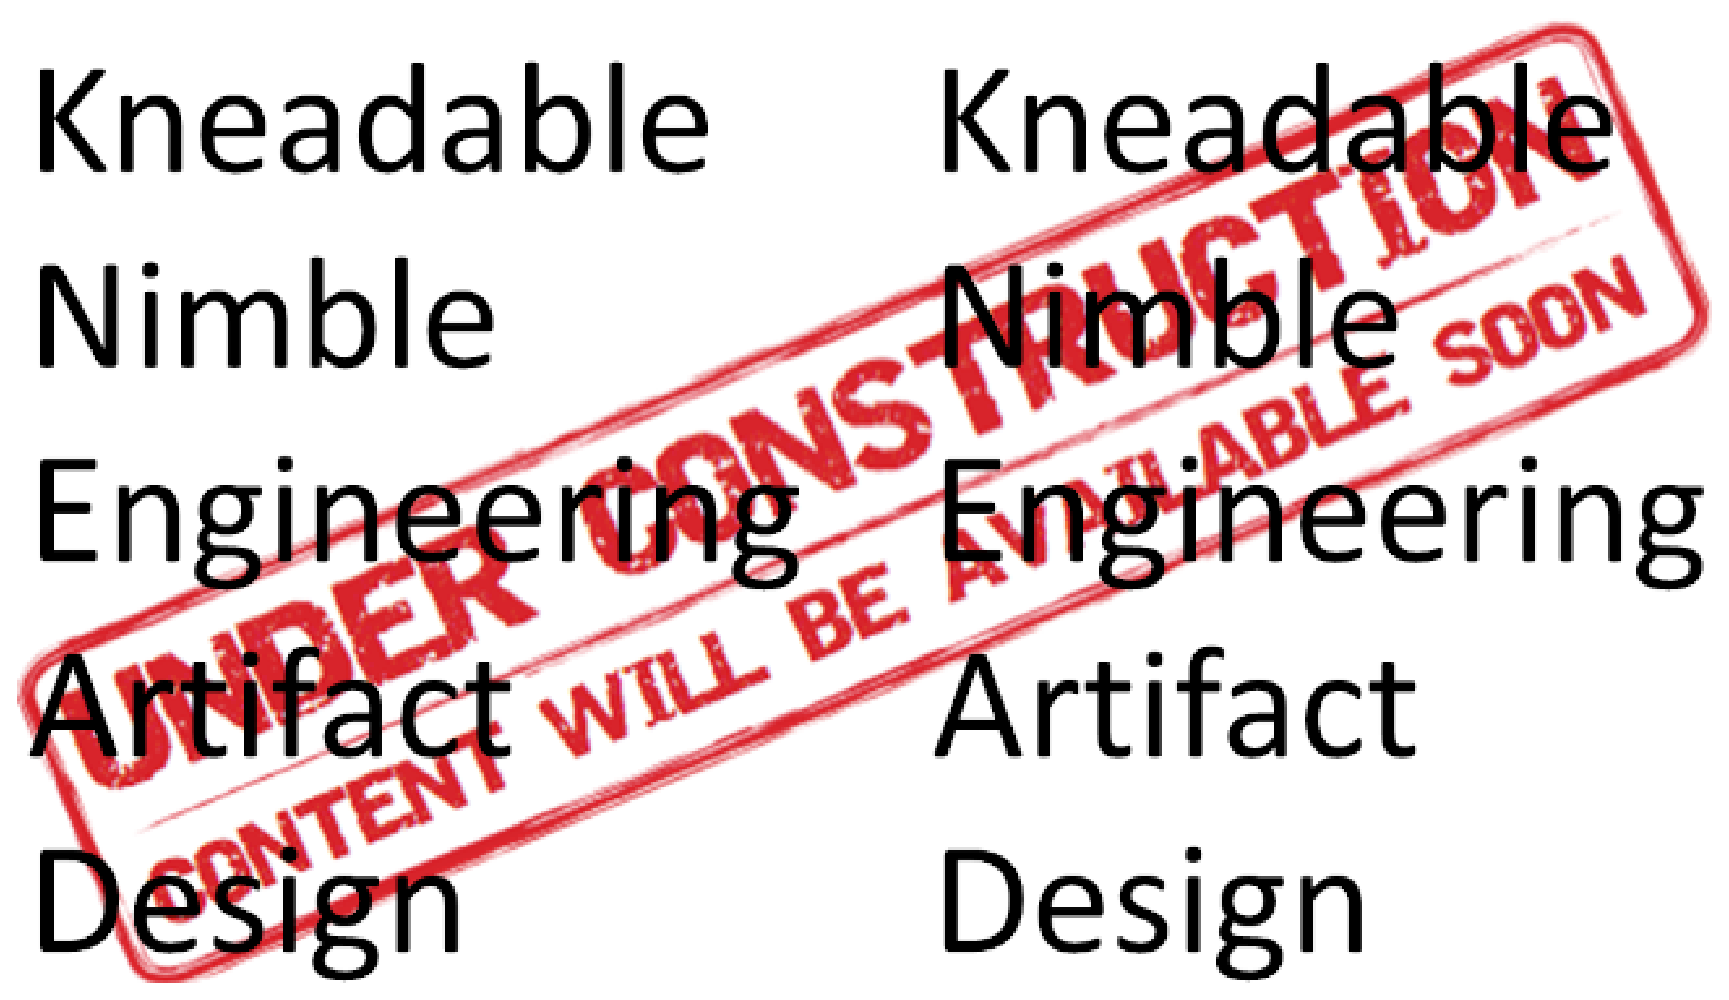
\includegraphics[width=6in]{images/KNEAD_UnderConstruction_100dpi_6.5inchesWide.eps}
		\caption{System Overview}
	\label{fig:SystemOverview}
\end{figure}
This diagram shows the major external interfaces that provide the capabilities of \ThisSys.
As are shown, the \ThisSys can provide. This system's main goal is to automate functionality
in order to make great Espresso.


The general concept of operations (\CONOP) for this system is User Selects an input weight through
an OLED screen using a rotery encoder. Espresso is prepared. User begins a shot, solid state relays 
are enabled and the shot begins to pull and a timer is started. As water falls into the cup and onto 
the load cells, the espresso cup is weighed. Once the desired weight is met the pump is turned off.
The user is displayed their time and weight on the OLED screen and data is pushed \TBD

While the system is not actively pulling a shot, it will be monitoring the water level. If low water
is detected the user will be notified.





